% Paper 1 -- ICAIIT 2027, Track 8 (Digital Economy, Business Informatics and Information Systems)
% Compile: pdflatex main.tex (twice). Anonymous submission copy: \documentclass[review]{icaiit2027}
\documentclass{icaiit2027}

\title{A Risk-Tiered Language Model Agent for Small Business Workflow Automation with Validated Tool Calls}
\icaiitauthors{Ahmed Ali and Asher Mehfooz}
\icaiitaffiliations{University of Kotli Azad Jammu and Kashmir, Kotli 11100, Azad Jammu and Kashmir, Pakistan\\
rajaahmedalikhan97@gmail.com, info.hasher@gmail.com}

\keywords{Language Model Agents, Tool Calling, Business Process Automation, Human-in-the-Loop, Input Validation.}

\abstract{Small businesses are adopting language-model agents that act on business records: they issue refunds, cancel orders, update customer notes, and send e-mails. Demonstrations look convincing until the model calls a tool with a malformed argument, refunds an order that belongs to someone else, or acts on a request that no policy covers. Common agent frameworks execute whatever call the model emits, while recent governed-execution systems target large regulated back offices and report few measurements that a small firm can reproduce. This paper treats the model as an untrusted planner. It may only propose a JSON tool call; deterministic code checks the call's schema, its evidence, record ownership, and business policy before anything runs, and calls that pass are routed by risk tier to automatic execution, one-click confirmation, or a typed reason. We evaluate the design on a public synthetic store with six tools and 100 scripted customer tickets, 36 of which should be escalated rather than executed, using two small open models running on a laptop CPU. Executing the planner's calls directly produces a wrong state change on 20 of 100 tickets with Phi-3.5-mini, including refunds outside the policy window, cancellations of dispatched orders, and refunds of other customers' orders. The validator removes 15 of those 20 and blocks none of the 60 correct calls once free-text fields are checked tolerantly; a strict variant blocks 18 correct calls. The remaining 5 wrong calls are policy gaps that the tiers send to a human. A second planner, Phi-3-mini, gives the same picture, and neither model ever chose to escalate by itself. The contribution is a reproducible validator-first design and a measurement of which errors it removes, not a new model.}

\begin{document}
\maketitle

\section{Introduction}

A language-model agent in a small business is valuable only if it touches records. Answering a question about the refund policy saves little time; issuing the refund does. The same step creates the risk. The failure of such an agent is rarely a badly worded paragraph. It is a bad tool call: a refund to the wrong order, a cancellation after dispatch, an apology e-mail to a customer who asked for compensation that no policy grants. Each of these is syntactically plausible, and each changes the state of the business.

Agent frameworks built around reasoning-and-acting loops \cite{yao2023} and tool-use training \cite{schick2023,qin2024} make it easy to connect a model to an API. In the default configuration the framework executes what the model emits. Tool hallucination, including invented tools, wrong parameters, and misread outputs, is documented in dedicated benchmarks \cite{patil2023,zhang2024}. Human approval queues are the common remedy, but people who confirm machine proposals under time pressure drift into complacency and automation bias \cite{parasuraman2010,goddard2012}. A checkbox is not a validator.

This paper studies a small, reproducible alternative. The model is an \emph{untrusted planner}: it may only propose one JSON call per ticket. Deterministic code, which the business owner can read, decides whether that call may run and who must look at it first. We ask three questions. (1) Which errors of a small open model does a deterministic validator remove before execution? (2) What does the validator cost in correct actions that it blocks? (3) After validation, how much work and how much residual risk reach the human approver?

The contributions are an implementation of a validator-first, risk-tiered agent for small-business workflows; a public ticket set with gold actions, including tickets that must be escalated; and a measurement of wrong state changes, blocked correct calls, and approval load with two small language models running on a laptop CPU. We do not claim the first governed enterprise agent, and we do not compare against systems for regulated back offices on their own tasks.

Section~2 reviews related work. Section~3 describes the system. Section~4 describes the store, the tickets, and the metrics. Section~5 reports results, Section~6 discusses limits, and Section~7 concludes.

\section{Related Work}

\subsection{Tool-Using Language Models}

ReAct interleaves reasoning traces with actions \cite{yao2023}, Toolformer teaches a model to insert API calls \cite{schick2023}, and ToolLLM scales tool use to thousands of real APIs \cite{qin2024}. Multi-agent frameworks such as AutoGen orchestrate several such agents \cite{wu2023}, and domain platforms such as FinRobot map financial tasks to agent workflows \cite{yang2024}. AgentBench evaluates models as agents across environments \cite{liu2024}. These works measure whether an agent completes tasks. They mostly assume that the environment will accept or reject a call on its own.

\subsection{Tool Errors and Agent Risk}

Gorilla shows that models hallucinate API calls and that retrieval of documentation reduces the problem \cite{patil2023}. ToolBeHonest diagnoses hallucination in tool-augmented models at several levels, including unsolvable requests \cite{zhang2024}. ToolEmu uses a language model to emulate tool execution and to identify risky agent actions \cite{ruan2024}. Prompt injection through retrieved content can make an agent call tools against the user's interest \cite{greshake2023,debenedetti2024}. Guided generation can force a model's output to match a schema \cite{willard2023}, which removes malformed JSON but cannot tell whether a well-formed refund is allowed.

\subsection{Governed Execution}

Two recent systems are closest to this work. POLARIS synthesises typed plans for back-office finance tasks and guards execution with validator-gated checks, a bounded repair loop, and compiled policy guardrails \cite{moslemi2026}. Bounded autonomy constrains a deployed multi-tenant enterprise application through typed action contracts, permission-aware capability exposure, and consumer-side execution, and compares manual, unconstrained, and bounded operation over 25 scenario trials \cite{sohail2026}. Table~\ref{tab:related} positions our work. It is smaller than both, targets a small firm without a platform team, publishes its ticket set with gold actions, and measures what reaches the human approver.

\begin{table*}[t]
  \caption{Comparison with related agent work. Gate: checks before execution. Tiers: routing of validated actions by risk. Public tasks: tasks released with gold actions. Approval load: measurement of what reaches a human.}
  \label{tab:related}
  \centering\footnotesize
  \begin{tabular}{@{}l l l l l@{}}
    \toprule
    Work & Gate & Tiers & Public tasks & Approval load \\
    \midrule
    AutoGen, ReAct \cite{wu2023,yao2023} & no & no & no & no \\
    Gorilla, ToolBeHonest \cite{patil2023,zhang2024} & no & no & benchmark & no \\
    ToolEmu \cite{ruan2024} & LM-emulated sandbox & no & benchmark & no \\
    POLARIS \cite{moslemi2026} & validator-gated checks & policy routing & synthetic suite & no \\
    Bounded autonomy \cite{sohail2026} & typed action contracts & permissions & no & no \\
    This paper & five-layer validator & read / update / money & 100 tickets & yes \\
    \bottomrule
  \end{tabular}
\end{table*}

\section{System}

Figure~\ref{fig:arch} shows the architecture. A ticket reaches the planner; the planner's proposal reaches the validator; only a validated proposal reaches a risk tier; and only the tier decides whether a person must act before the business API runs.

\begin{figure*}[t]
  \centering
  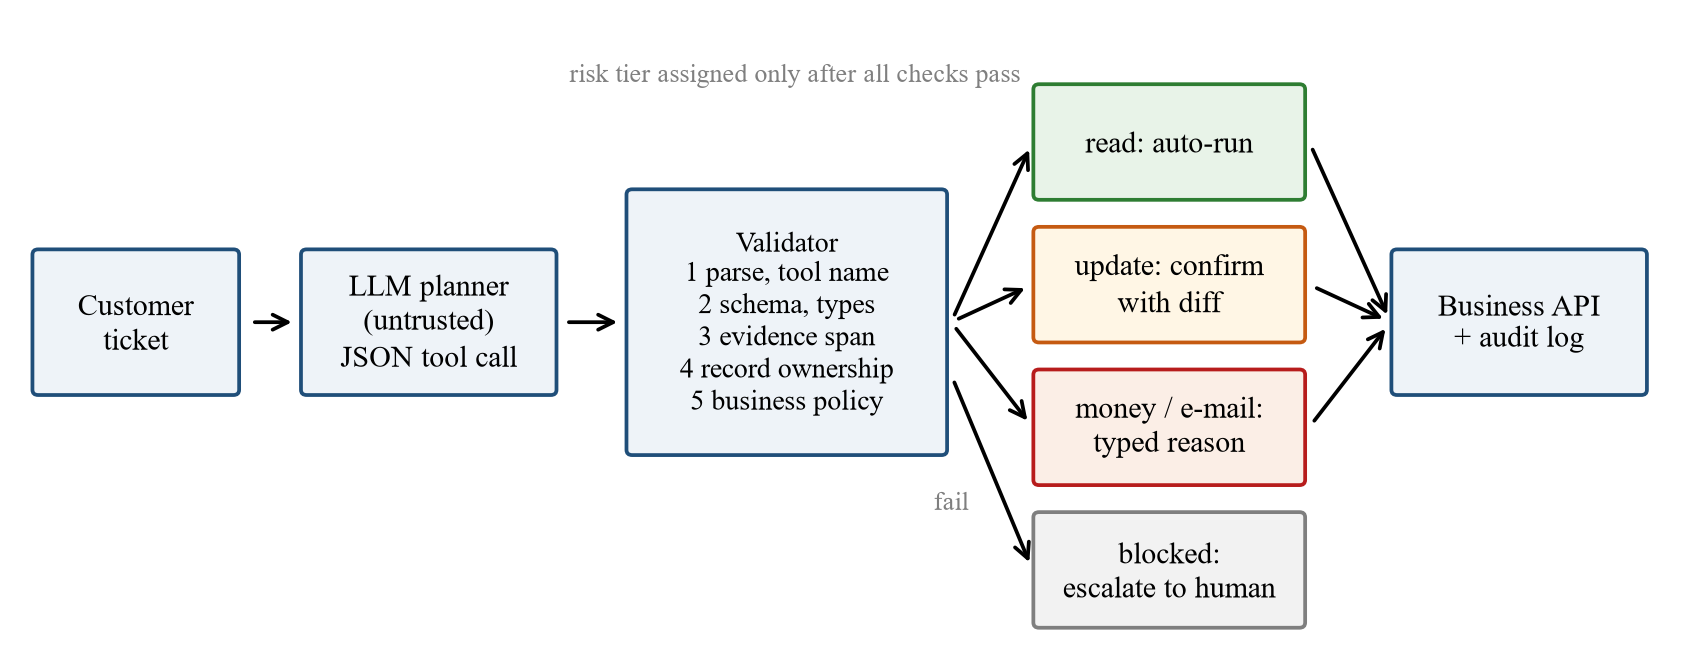
\includegraphics[width=0.9\textwidth]{figures/fig1_architecture.png}
  \caption{Validator-first agent. The planner can only propose; checks run before any tier, and a failed check becomes an escalation.}
  \label{fig:arch}
\end{figure*}

\subsection{Planner}

The planner is a small instruction-tuned language model prompted with the tool list, the argument types, four lines of shop policy, and one customer ticket. It must answer with one JSON object \{tool, args, evidence\_span\}, where the evidence span is text copied from the ticket that justifies the call. The prompt tells the model to escalate when the policy does not cover the request. Decoding is greedy. Nothing the planner emits is executed directly. Listing~\ref{lst:call} shows a real proposal from the evaluation: well formed, grounded in a verbatim quote, and wrong, because order O1042 belongs to a different customer.

\begin{listing}[t]
\begin{algobody}
ticket from C032:
\ind"Refund order O1042 please, the item
\ind was not what I expected."
planner:
\{"tool": "refund",
\ind"args": \{"order\_id": "O1042",
\ind\ind"amount": 39.00,
\ind\ind"reason":
\ind\ind\ind"item not as expected"\},
\ind"evidence\_span":
\ind\ind"Refund order O1042 please, ..."\}
validator:
\ind reference: order belongs to C031
\end{algobody}
\caption{A planner proposal blocked by the ownership check.}
\label{lst:call}
\end{listing}

\subsection{Validator}

The validator runs five layers in a fixed order and stops at the first failure. (1) \emph{Parse}: the output must contain a JSON object with a known tool name. (2) \emph{Schema}: required arguments must be present with the right types and no unknown arguments may appear. (3) \emph{Evidence}: the evidence span must occur in the ticket, and any order identifier must appear in the ticket text. (4) \emph{Reference}: the order must exist and belong to the ticket's sender, and a customer identifier must equal the sender. (5) \emph{Policy}: a cancellation requires an undispatched order; a refund requires a delivered order, an amount between zero and the unrefunded total, and delivery within 14 days, or 60 days when the ticket reports damage; an order needs a known product and a quantity from 1 to 10; an e-mail needs an approved template. A failed call becomes an escalation with the failing layer recorded.

We evaluate two settings of the free-text checks. The \emph{strict} validator requires the \emph{reason} argument and an exact evidence substring. The \emph{tolerant} validator accepts a missing reason and a missing or reordered evidence span as long as at least 80\% of its words occur in the ticket. Reference and policy checks are identical in both.

\subsection{Risk Tiers}

A call that passes the validator is assigned a tier by its tool. \emph{Read} calls (order lookup) and escalations run automatically. \emph{Update} calls (create order, cancel order, customer note) wait for a one-click confirmation that shows the record diff. \emph{Money} calls, which here include refunds and outbound customer e-mail because neither can be taken back, wait for the approver to type a reason. The tier is a property of the action, not of the model's confidence, so the planner cannot talk its way into a lower tier.

\subsection{Audit Log}

Every proposal is appended to a JSON-lines log with the raw model output, the validator layer and message, and the tier. The log is the evidence an owner needs when a customer disputes an action, and it is the data source for all numbers in Section~5.

\section{Experimental Setup}

\subsection{Synthetic Store}

The store is generated from a fixed seed: 40 customers, 70 orders over eight products, each order placed, dispatched, or delivered between 1 and 45 days before a fixed evaluation date. The business API offers six tools plus escalation and behaves like a typical CRUD backend: it fails on missing records and non-numeric amounts, but it enforces no business policy. That is the realistic baseline for a small firm whose API was written before any agent existed.

\subsection{Ticket Set}

The 100 tickets are generated from templates over the store records and cover ten situations (Table~\ref{tab:tickets}). Each ticket has a gold action: a tool with key arguments, or \emph{escalate} when the correct system behaviour is to execute nothing. Thirty-six tickets are escalation cases: refunds outside the 14-day window, cancellations after dispatch, refund requests naming another customer's or a non-existent order, and requests that no policy covers (an international warranty, a price match, instalments, compensation for a rude courier). The set is published with the code.

\begin{table}[t]
  \caption{Ticket set: situations, counts, and gold action.}
  \label{tab:tickets}
  \centering\footnotesize
  \setlength{\tabcolsep}{3pt}
  \begin{tabularx}{\columnwidth}{@{}X r l@{}}
    \toprule
    Situation & $n$ & Gold action \\
    \midrule
    Order status question & 14 & get\_order \\
    Unopened refund within 14 days & 14 & refund \\
    Damaged item refund & 10 & refund \\
    Cancel before dispatch & 12 & cancel\_order \\
    Address or contact note & 8 & update\_crm\_note \\
    Re-order a product & 6 & create\_order \\
    Unopened refund after 14 days & 12 & escalate \\
    Cancel after dispatch & 8 & escalate \\
    Wrong or foreign order ID & 8 & escalate \\
    Request not covered by policy & 8 & escalate \\
    \bottomrule
  \end{tabularx}
\end{table}

\subsection{Planners, Conditions, and Metrics}

Two planners are used: Phi-3.5-mini-instruct and Phi-3-mini-4k-instruct \cite{abdin2024}, both in 4-bit quantisation, run with ONNX Runtime on an AMD Ryzen 5 7430U laptop CPU with 8 GB of memory and no GPU. Each ticket receives one planner proposal, and the same proposal is evaluated under three conditions: (A) \emph{unconstrained}, where the call is sent straight to the API; (B) \emph{validator}, strict and tolerant; and (C) \emph{validator plus tiers}.

A proposal is \emph{correct} if its tool and key arguments equal the gold action. Outcomes are counted per ticket: a correct action; a \emph{wrong state change}, meaning an executed call that changes records and is not the gold action; a \emph{failed call} that the API rejects; a \emph{correct block} of a wrong call; and an \emph{overblock} of a correct call. For condition C we report how many actions reach each tier and how many wrong actions sit in the human queue.

\section{Results}

\subsection{What the Planner Proposes}

Phi-3.5-mini proposed the gold action on 60 of 100 tickets at 9.7~s per ticket. It never invented a tool name, and only one output was not parseable JSON. Its errors were of a different kind. It wrote amounts as text (``full price of the usb-c hub'') on 12 tickets, omitted the required reason on 4, and added an unsupported argument on 3. Most importantly, it never chose \emph{escalate}: on all 36 escalation tickets it proposed an action. A small planner, even with an explicit instruction to escalate, acts.

\subsection{Unconstrained Execution}

Sent directly to the API, the proposals produced 60 correct actions, 20 failed calls, and 20 wrong state changes (Figure~\ref{fig:outcomes}). The wrong state changes are exactly the cases a small business fears: 8 cancellations of already dispatched orders, 4 refunds of orders that belong to another customer, 3 refunds outside the 14-day window, 4 apology e-mails sent in reply to compensation requests, and 1 customer note recording a warranty question as if it were an action. The 20 failed calls were rejected by the API only by accident: a non-numeric amount, an unknown product, or a non-existent order raised an error. Nine of them were late refunds that would have executed wrongly had the model written the amount as a number.

\begin{figure}[t]
  \centering
  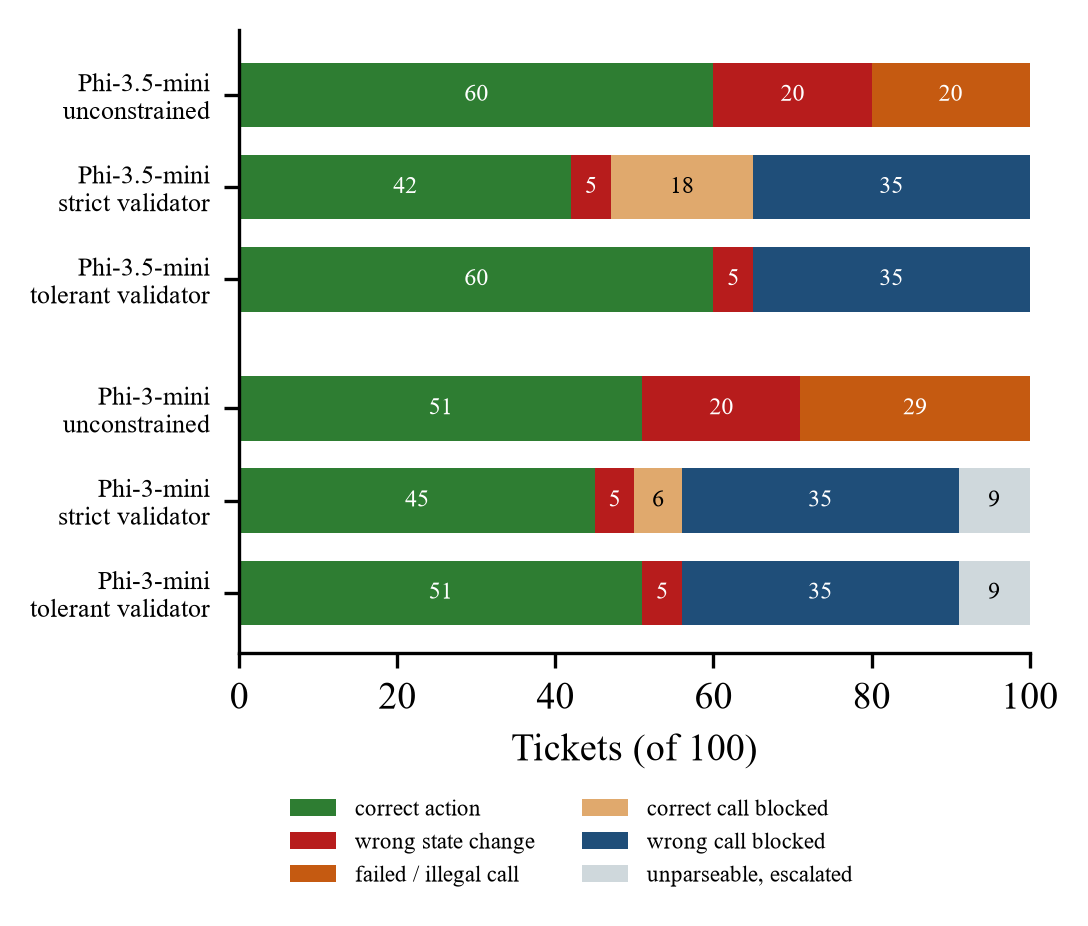
\includegraphics[width=\columnwidth]{figures/fig2_outcomes.png}
  \caption{Outcomes per ticket under the three conditions for both planners.}
  \label{fig:outcomes}
\end{figure}

\subsection{Validator}

The strict validator blocked 53 proposals. Thirty-five of them were wrong calls, so the validator removed 15 of the 20 wrong state changes and all 20 failed calls. The other 18 blocks were correct calls that failed only the free-text checks: 15 had a missing or reordered evidence span and 3 lacked the reason argument. Table~\ref{tab:results} summarises the conditions.

\begin{table}[t]
  \caption{Outcomes on 100 tickets with the Phi-3.5-mini planner. Wrong = executed wrong state change.}
  \label{tab:results}
  \centering\footnotesize
  \setlength{\tabcolsep}{2.5pt}
  \begin{tabularx}{\columnwidth}{@{}X r r >{\raggedleft\arraybackslash}p{1.0cm} >{\raggedleft\arraybackslash}p{1.0cm}@{}}
    \toprule
    Condition & Correct & Wrong & Blocked wrong & Blocked correct \\
    \midrule
    A: unconstrained & 60 & 20 & -- & -- \\
    B: strict validator & 42 & 5 & 35 & 18 \\
    B: tolerant validator & 60 & 5 & 35 & 0 \\
    C: tolerant + tiers & 60 & 0 auto & 35 & 0 \\
    \bottomrule
  \end{tabularx}
\end{table}

The tolerant validator passed all 60 correct calls and still blocked the same 35 wrong ones. Its blocks come from the schema layer (15, mostly amounts written as text), the policy layer (11: eight cancellations of dispatched orders and three late refunds), the reference layer (8 refunds of foreign or non-existent orders), and one unparseable output. In this measurement the strict free-text checks cost 18 correct actions and bought no safety, because every wrong call that mattered was caught by the reference or policy layer. The design rule is to validate references and policy strictly and free text tolerantly.

Five wrong calls passed both validators: four \emph{delay\_apology} e-mails and one customer note, all on tickets that no policy covers. They are well-formed calls with approved templates and grounded evidence (``I want compensation''). A validator can check what a policy says; it cannot see that a request falls outside every policy unless the policy lists what is allowed for each request type.

\subsection{Risk Tiers and Approval Load}

With the tolerant validator, 14 read calls ran automatically and all were correct. Fifty-one actions reached a human: 27 update confirmations and 24 money approvals with a typed reason. No wrong state change ran without a person. The residual risk has moved, not vanished: 5 of the 51 queued actions are wrong, and all four wrong e-mails sit in the money tier. An approver sees nine correct actions for every wrong one. This is the setting in which automation bias is documented \cite{parasuraman2010,goddard2012}, and it is the argument for making the typed reason a question about the policy rather than a formality.

\subsection{A Second Planner}

The older Phi-3-mini-4k planner proposed the gold action on 51 tickets. It produced 12 unparseable outputs, often a JSON object that was never closed, and like Phi-3.5-mini it never invented a tool and never chose to escalate. Unconstrained, it caused 20 wrong state changes (8 late cancellations, 4 late refunds, 3 refunds of foreign orders, and the same 5 policy-gap actions) and 29 failed calls. Under the tolerant validator it kept all 51 correct actions, blocked the same 35 wrong calls, and let through the same 5 policy-gap calls on exactly the same tickets as the stronger planner; the 9 remaining tickets were unparseable outputs that became escalations. The strict validator again blocked correct calls, 6 this time, all for a missing evidence span. With the tolerant validator and tiers, 14 read calls ran automatically and 42 actions reached a human, 5 of them wrong. The validator's effect is therefore stable across planners: what changes between models is how many correct calls are available to pass, not which wrong calls get through.

\section{Discussion}

The results support three design rules for small-business agents. First, never let the planner's output reach the API directly; a CRUD backend rejects malformed calls by accident, not by policy. Second, check references and policy strictly and free text tolerantly. Third, decide the approval tier by the action's reversibility, and expect the human queue to be mostly correct items with rare, important exceptions.

\subsection{Limitations}

The store and tickets are synthetic and English-only, and the tickets are templated, so the planner sees less linguistic variety than a real inbox. One proposal per ticket is evaluated; a repair loop that returns the validator's message to the planner could recover some blocked calls and is future work. The damage rule uses a keyword list. No approver took part, so approval time and fatigue are proxies: we report queue size and the share of wrong items in it, not human decisions.

\subsection{Threats to Validity}

Gold actions encode one reading of the shop policy; another owner could treat a courier complaint differently. Both planners come from one model family, and larger models may escalate on their own. Correctness requires exact key arguments, which is strict for amounts but appropriate for money. All numbers are produced by scripts published with the ticket set.

\section{Conclusion}

A small open language model on a laptop can plan most routine business actions, but when its calls run unchecked it changes records wrongly on one ticket in five and never asks for help. A deterministic validator in front of the API removes three quarters of those wrong changes at no cost in correct actions, provided that free-text fields are checked tolerantly. Risk tiers ensure that nothing irreversible runs without a person. The errors that remain are requests outside every policy, and they end up in front of an approver who mostly sees correct items. The next step is to make that approval an explanation the worker can question, and to feed a calibrated intent classifier in front of the planner so that uncovered requests are escalated before a call is proposed.

\begin{thebibliography}{17}

\bibitem{yao2023} S. Yao et al., ``ReAct: Synergizing reasoning and acting in language models,'' in \emph{Proc. International Conference on Learning Representations}, 2023, doi: 10.48550/arXiv.2210.03629.

\bibitem{schick2023} T. Schick et al., ``Toolformer: Language models can teach themselves to use tools,'' in \emph{Advances in Neural Information Processing Systems}, vol. 36, 2023, doi: 10.48550/arXiv.2302.04761.

\bibitem{patil2023} S. G. Patil, T. Zhang, X. Wang, and J. E. Gonzalez, ``Gorilla: Large language model connected with massive APIs,'' arXiv preprint, 2023, doi: 10.48550/arXiv.2305.15334.

\bibitem{qin2024} Y. Qin et al., ``ToolLLM: Facilitating large language models to master 16000+ real-world APIs,'' in \emph{Proc. International Conference on Learning Representations}, 2024, doi: 10.48550/arXiv.2307.16789.

\bibitem{wu2023} Q. Wu et al., ``AutoGen: Enabling next-gen LLM applications via multi-agent conversation,'' arXiv preprint, 2023, doi: 10.48550/arXiv.2308.08155.

\bibitem{zhang2024} Y. Zhang et al., ``ToolBeHonest: A multi-level hallucination diagnostic benchmark for tool-augmented large language models,'' in \emph{Proc. Conference on Empirical Methods in Natural Language Processing}, 2024, pp. 11388--11422, doi: 10.18653/v1/2024.emnlp-main.637.

\bibitem{ruan2024} Y. Ruan et al., ``Identifying the risks of LM agents with an LM-emulated sandbox,'' in \emph{Proc. International Conference on Learning Representations}, 2024, doi: 10.48550/arXiv.2309.15817.

\bibitem{liu2024} X. Liu et al., ``AgentBench: Evaluating LLMs as agents,'' in \emph{Proc. International Conference on Learning Representations}, 2024, doi: 10.48550/arXiv.2308.03688.

\bibitem{moslemi2026} Z. Moslemi, K. Koneru, Y.-T. Lee, S. Kumar, and R. Radhakrishnan, ``POLARIS: Typed planning and governed execution for agentic AI in back-office automation,'' arXiv preprint, 2026, doi: 10.48550/arXiv.2601.11816.

\bibitem{sohail2026} S. Sohail and G. Haider, ``Bounded autonomy for enterprise AI: Typed action contracts and consumer-side execution,'' arXiv preprint, 2026, doi: 10.48550/arXiv.2604.14723.

\bibitem{yang2024} H. Yang et al., ``FinRobot: An open-source AI agent platform for financial applications using large language models,'' arXiv preprint, 2024, doi: 10.48550/arXiv.2405.14767.

\bibitem{greshake2023} K. Greshake, S. Abdelnabi, S. Mishra, C. Endres, T. Holz, and M. Fritz, ``Not what you've signed up for: Compromising real-world LLM-integrated applications with indirect prompt injection,'' in \emph{Proc. 16th ACM Workshop on Artificial Intelligence and Security}, 2023, pp. 79--90, doi: 10.1145/3605764.3623985.

\bibitem{debenedetti2024} E. Debenedetti, J. Zhang, M. Balunovi\'{c}, L. Beurer-Kellner, M. Fischer, and F. Tram\`{e}r, ``AgentDojo: A dynamic environment to evaluate prompt injection attacks and defenses for LLM agents,'' in \emph{Advances in Neural Information Processing Systems}, vol. 37, 2024, doi: 10.48550/arXiv.2406.13352.

\bibitem{parasuraman2010} R. Parasuraman and D. H. Manzey, ``Complacency and bias in human use of automation: An attentional integration,'' \emph{Human Factors}, vol. 52, no. 3, pp. 381--410, 2010, doi: 10.1177/0018720810376055.

\bibitem{goddard2012} K. Goddard, A. Roudsari, and J. C. Wyatt, ``Automation bias: A systematic review of frequency, effect mediators, and mitigators,'' \emph{Journal of the American Medical Informatics Association}, vol. 19, no. 1, pp. 121--127, 2012, doi: 10.1136/amiajnl-2011-000089.

\bibitem{abdin2024} M. Abdin et al., ``Phi-3 technical report: A highly capable language model locally on your phone,'' arXiv preprint, 2024, doi: 10.48550/arXiv.2404.14219.

\bibitem{willard2023} B. T. Willard and R. Louf, ``Efficient guided generation for large language models,'' arXiv preprint, 2023, doi: 10.48550/arXiv.2307.09702.

\end{thebibliography}


\end{document}
